% Chapter 1 -- structure from table of content.md; writing style from README_STYLE_PFE.md

\reportchapter{1}{Context and State of the Art}{Institutional context, project motivation, theoretical foundations, and research positioning.}

\section{Introduction}

In this chapter, the end-of-study internship is situated within the research environment of the host organization, SCIENTIAE, and the theoretical background required to understand the platform developed during the PFE is reviewed. The chapter first presents the company and the constraints of political intelligence analysis, then surveys large language models, retrieval-augmented generation, knowledge graphs, political NLP, and reasoning paradigms. It closes by stating the research gap and the positioning of the project. This progression moves from institutional context to scientific foundations before Chapter~2 formalizes requirements, actors, and validation criteria.

\section{Host Organization Overview}

\subsection{Company Profile}

This graduation project took place at \textbf{SCIENTIAE}, the host organization in Rabat. Before the technical chapters, it is useful to recall the institutional setting in which the platform was designed, tested, and progressively enriched with real political data.

\begin{figure}[H]
    \centering
    \vspace{1cm}
    
\includegraphics[height=1.5cm]{Logos/Company_Logo_Scientiae.png}
    \caption{SCIENTIAE, host organization of the end-of-study internship.}
    \label{fig:host-organization}
    \vspace{1cm}
\end{figure}

SCIENTIAE is an emerging company based in Hay Riad, Rabat, oriented towards high-tech activities in data, security, and digital solutions. Its offering is centered on consulting, support, and tailored solution design, with a commitment to service quality, industry standards, and innovation.

Beyond this profile, SCIENTIAE provides a favorable environment for exploratory engineering work in software engineering, data processing, automation, and knowledge valuation. This context offered technical autonomy and a clear application domain for a platform devoted to extracting, enriching, and structuring knowledge from heterogeneous textual sources. The PFE therefore fits the company's R\&D strategy aimed at sovereign decision-intelligence solutions for institutional partners.

\subsection{Organizational Structure}

The internal organization of SCIENTIAE is summarized below to clarify how the project was supervised and integrated. The company is structured around a General Management from which two major poles are deployed: an Administrative Department (Human Resources, Finance) and a Research and Development Department coordinating software engineering, data science engineering, and cybersecurity engineering.

\begin{figure}[H]
    \centering
    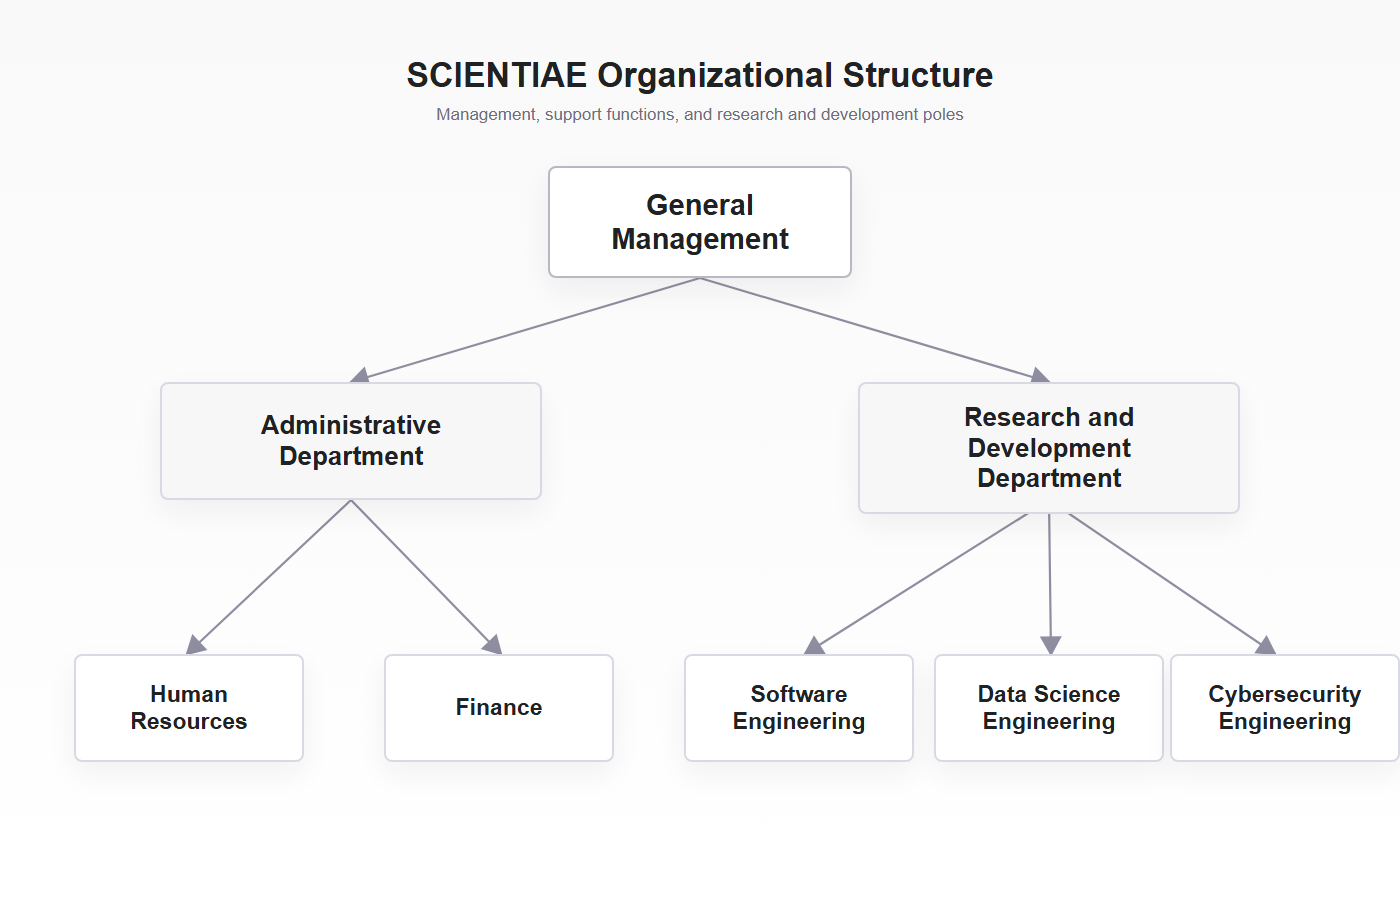
\includegraphics[width=0.96\textwidth,height=0.78\textheight,keepaspectratio]{images/org_chart.png}
    \caption{Organizational structure of SCIENTIAE.}
    \label{fig:org-chart}
\end{figure}

Figure~\ref{fig:org-chart} summarizes this organization. The project was anchored in the R\&D pole, which facilitated regular exchanges with profiles specialized in data and platform development. The internship was conducted under academic supervision at INPT and professional supervision at SCIENTIAE, with periodic reviews of progress, architecture choices, and demonstration milestones. The technical stack, component boundaries, and deployment choices are detailed in Chapters~3 and~4 rather than in this contextual section.

\subsection{Services and R\&D Focus}

The R\&D pole combines three complementary professions that shaped the orientation of the project. Cybersecurity supports the protection of information systems and incident monitoring. Web development covers application services, hosting, and user interfaces. Data science, the most central orientation here, focuses on structuring and exploiting large volumes of data to extract actionable knowledge. A knowledge-graph approach follows this logic: political documents are transformed into structured evidence that can be queried, explored, and reasoned over.

From a technological perspective, the internship mobilized a modern data-and-AI stack rather than a monolithic toolchain. Figure~\ref{fig:tech-overview} illustrates representative components: Python and FastAPI for backend services, React for the analytical interface, DSPy for structured LLM orchestration \cite{khattab-dspy}, and containerized deployment for reproducibility. The platform also relies on document, graph, vector, and cache stores, together with observability tooling. These families are introduced here only as context; versions, APIs, schemas, and engineering trade-offs are presented in the design and implementation chapters.

\begin{figure}[H]
    \centering
    \raisebox{-0.15\height}{
\includegraphics[height=0.95cm]{Logos/python.png}}\hspace{0.6cm}
    \raisebox{-0.15\height}{
\includegraphics[height=0.95cm]{Logos/fastapi.png}}\hspace{0.6cm}
    \raisebox{-0.15\height}{
\includegraphics[height=0.95cm]{Logos/react.png}}\hspace{0.6cm}
    \raisebox{-0.15\height}{
\includegraphics[height=0.95cm]{Logos/dspy_logo.png}}
    \caption{Representative technologies of the R\&D environment (detailed architecture in Chapters~3--4).}
    \label{fig:tech-overview}
\end{figure}

This overview clarifies why the PFE could be conducted as applied research with industrial constraints rather than as a purely theoretical study. The following section addresses the political intelligence context that motivated the platform.

\section{Project Context and Motivation}

\subsection{Political Intelligence Challenges}
\label{sec:political-intelligence-challenges}

Political intelligence targets a domain where information is abundant but difficult to exploit reliably. Analysis requires connecting actors, institutions, events, alliances, and temporal changes that are rarely stated explicitly in a single document. Keyword search and classical retrieval-augmented generation remain weak when the question depends on entity disambiguation, multi-hop relations, or temporal consistency.

Three recurring limitations motivate a hybrid architecture. First, flat retrieval cannot navigate explicit relationships between actors. Second, surface forms such as ``The President'' and ``Macron'' may be treated as distinct entities without resolution. Third, standard RAG often treats retrieved chunks as equally current, which leads to temporal drift when political positions evolve. These constraints are developed further in the state of the art and translated into requirements in Chapter~2.

\subsection{Data Volume and Heterogeneity}

Before any reasoning layer can operate, a political intelligence platform must obtain a reliable and continuously updated corpus. Web crawling is therefore a foundational requirement rather than a peripheral utility. Unlike large-scale search engines, the objective is constrained: prioritize relevant sources, preserve provenance, avoid duplicates, and produce clean documents for downstream NLP extraction.

The target platform must support complementary collection strategies: curated monitoring of RSS feeds and official portals; query-driven discovery through news aggregators; and document-oriented ingestion of PDF reports. Operational supervision (scheduling, manual triggers, logs) is also required so that freshness does not compromise control. Unlike approaches centered on a fixed external knowledge base, the PFE aims at a system that builds its own corpus and then extracts graph knowledge from collected evidence. The engineering realization of these ingestion levels is described in Chapter~4.

\subsection{Need for Evidence Traceability}

Autonomous crawling introduces a quality challenge that differs from classical information retrieval. A crawler decides what enters the corpus, which affects extraction quality, graph reliability, retrieval precision, and answer faithfulness. Traceability therefore requires preserving source URL, source name, topic, publication date, scraping date, language, and quality indicators, together with deduplication to limit syndication bias.

Another principle is to separate acquisition from interpretation: collection should remain broad, while extraction and graph publication decide whether a document contains political entities, relations, or events worth keeping. Table~\ref{tab:crawler-positioning} compares the \emph{design target} of the platform with common acquisition approaches. In the table, ``real-time updates'' for curated RSS means scheduled refresh of known feeds, not unconstrained open-web recrawl.

\begin{table}[H]
\centering
\scriptsize
\renewcommand{\arraystretch}{1.25}
\begin{tabularx}{\textwidth}{@{}>{\bfseries\raggedright\arraybackslash}p{3.1cm}XXXX@{}}
\toprule
\rowcolor{lightblue}
Approach & Source Coverage & Format Handling & Freshness & Operational Control \\
\midrule
Manual collection & Limited to analyst effort & Depends on user work & Irregular & No automation \\
Simple RSS reader & Curated feeds only & RSS summaries and linked articles & Scheduled feed refresh & Limited monitoring \\
One-shot web scraper & Targeted pages & Usually HTML only & Poor after execution & Weak supervision \\
External knowledge base & Structured reference data & Already normalized & Not focused on breaking news & Dependent on external updates \\
\textbf{Platform design target} & RSS, news discovery, direct URLs, PDF sources & HTML, RSS, PDF, normalized records & Scheduled and triggerable collection & Supervised dashboard and logs \\
\bottomrule
\end{tabularx}
\caption{Positioning of the platform ingestion design against common acquisition approaches.}
\label{tab:crawler-positioning}
\end{table}

The table highlights a deliberate choice: political intelligence depends on freshness, provenance, format diversity, and supervision rather than on a single channel. Manual collection and simple RSS readers lack operational depth; one-shot scrapers degrade over time; external knowledge bases are strong on structure but weak on breaking news under local control. The platform design target combines broader coverage with supervisable ingestion, at the cost of higher engineering complexity. Having established this context, the following section reviews the scientific foundations that informed the architectural choices retained for the platform.

\section{State of the Art}

\subsection{Large Language Models}

Large language models (LLMs) are neural sequence models based on the Transformer architecture \cite{vaswani-attention}. Self-attention computes, for each token, a weighted combination of all other token representations, which enables long-context modeling and parallel training at scale. This mechanism underpins contemporary extraction, classification, and answer synthesis pipelines.

Several model families are discussed in the literature and in industrial practice. Proprietary models such as GPT-4 offer strong reasoning but raise privacy and data-sovereignty concerns for sensitive political analysis. Open-weight families such as LLaMA~3 reduce vendor lock-in but may require substantial local GPU resources at scale. European foundation models such as Mistral Large are often selected when regulatory alignment and API governance matter. Independently of the vendor, LLMs remain subject to hallucination and to knowledge cutoffs unless generation is grounded in external retrieval \cite{lewis-rag}.

For the PFE, these observations justify an architecture where the LLM is not the sole source of truth. Parametric knowledge is complemented by retrieved documents, graph facts, and explicit citations, as developed in the following subsections.

\subsection{Retrieval-Augmented Generation (RAG)}

Retrieval-Augmented Generation (RAG) augments LLM generation with dynamically retrieved external knowledge \cite{lewis-rag}. The classical pipeline indexes documents by chunking and embedding them, retrieves the top-$k$ relevant passages for a query, and conditions answer generation on that evidence. This workflow is efficient for direct factual questions but structurally limited for relational political analysis, as noted in Section~\ref{sec:political-intelligence-challenges}.

Recent extensions focus on \textbf{evidence grounding and citation}: retrieved passages are linked to sources, incomplete evidence triggers additional retrieval, and confidence checks reduce unsupported synthesis. These mechanisms do not replace RAG; they make generation auditable, which is essential when answers may influence interpretation of institutions, actors, or conflicts. Grounding also prepares the transition to graph-backed retrieval, where evidence includes explicit relations rather than isolated text spans.

\subsection{Knowledge Graphs and Graph-RAG}

Classical RAG retrieves passages through semantic similarity. Graph-RAG constructs graph-structured knowledge from a corpus and retrieves through entities, relationships, communities, and source passages \cite{edge-graphrag,microsoft-graphrag}. Figure~\ref{fig:rag-vs-graphrag} contrasts the two retrieval paths and shows why geopolitical questions often require relational traversal.

\begin{figure}[H]
    \centering
    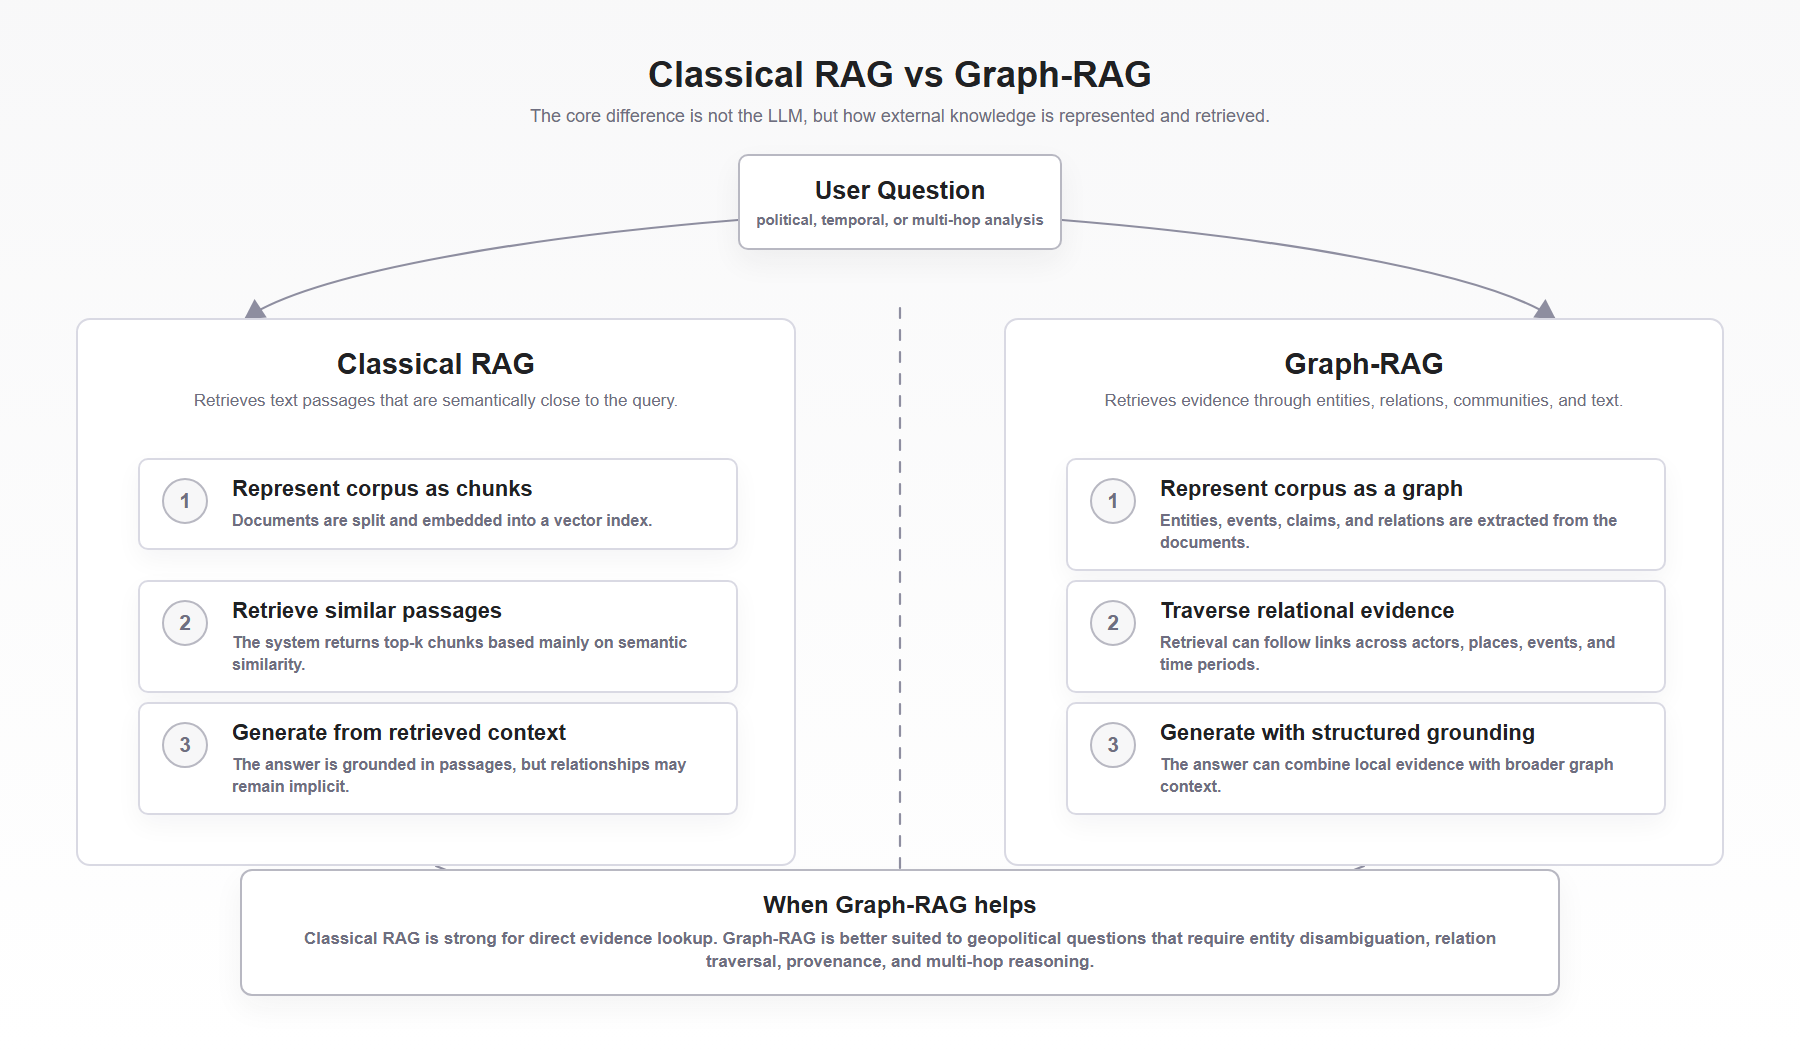
\includegraphics[width=0.96\textwidth,height=0.78\textheight,keepaspectratio]{images/rag_vs_graphrag.png}
    \caption{Comparison between classical RAG and Graph-RAG retrieval paths.}
    \label{fig:rag-vs-graphrag}
\end{figure}

\textbf{Knowledge graph concepts.} A knowledge graph represents entities and typed relations, optionally with temporal or provenance metadata. It supports entity disambiguation, path queries, and hybrid retrieval that combines vector similarity with structural constraints.

\textbf{Graph construction from text.} Pipelines typically perform extraction, entity resolution, and provenance linking so that each relation remains traceable to a source document. Noise control is critical because LLM-based extraction can introduce spurious nodes or edges if resolution rules are weak.

\textbf{Graph-RAG retrieval and reasoning.} Once published, the graph enables multi-hop traversal, community summarization, and fusion with textual chunks retrieved by dense search \cite{edge-graphrag,microsoft-graphrag}. This combination is particularly relevant when answers depend on chains of actors and events rather than on a single paragraph.

\subsection{LLM Reasoning and Thinking Modes}

Beyond retrieval format, recent work studies how a language model \emph{uses} evidence during generation. Classical RAG follows a mostly linear pipeline: retrieve once, then generate. This design is efficient for localized factual questions, but it is structurally weak when a query requires several retrieval steps, intermediate planning, or verification of partial evidence \cite{lewis-rag}.

\textbf{Chain-of-Thought and query decomposition.} Chain-of-Thought (CoT) prompting asks the model to produce intermediate reasoning steps before the final answer \cite{wei-cot}. In retrieval settings, decomposition splits a complex question into sub-questions and guides evidence collection step by step. The goal is not longer answers for their own sake, but better coverage when the first retrieved batch is incomplete.

\textbf{Interleaved retrieval and multi-hop reasoning.} IRCoT interleaves retrieval with ongoing chain-of-thought generation: each reasoning step can trigger a new retrieval call guided by what was learned in the previous step \cite{trivedi-ircot}. This pattern is especially relevant for multi-hop questions where bridge entities only become visible after an initial pass. When knowledge is graph-structured, multi-hop traversal plays a similar role by following explicit paths between actors and events rather than relying on lexical similarity alone.

\textbf{ReAct and tool-interleaved control.} ReAct combines reasoning traces with actions such as search, graph lookup, or tool invocation \cite{yao-react}. Instead of a fixed retrieve-then-generate sequence, the model alternates between thinking steps and operations on external memory. This architecture is a precursor to modern agentic pipelines in which a controller decides when to retrieve again, when to stop, and when to synthesize.

\textbf{Reflection and Self-RAG.} Reflection-based methods add a critique step that evaluates whether the current evidence supports the draft answer. Self-RAG trains the model to decide when retrieval is needed, when generation is sufficient, and when the output should be revised \cite{asai-selfrag}. These approaches reduce unsupported synthesis at the cost of additional model calls and higher latency.

\textbf{Agentic RAG.} Agentic RAG generalizes the above patterns into loops that may include planning, routing, iterative retrieval, critique, and final synthesis. Surveys of the field describe a recurring trade-off: iterative and reflective pipelines improve faithfulness on relational or multi-step tasks, but they increase token cost and response time compared with naive RAG. For political intelligence, this literature motivates architectures in which reasoning depth can be adapted to question complexity rather than forcing every query through the heaviest pipeline.

Chapter~4 presents the reasoning modes implemented in the platform and describes how these ideas are operationalized in production.

\subsection{Political NLP and Temporal Modeling}

Political NLP extends language understanding to actors, institutions, stances, conflicts, and temporal relations. \textbf{Entity and relation extraction} increasingly relies on joint models that predict tuples under schema constraints, reducing error propagation compared with rigid pipelines. \textbf{Stance and conflict analysis} aims to detect how an actor relates to a target event or entity; zero-shot and weakly supervised methods are common when labeled political data are scarce \cite{allaway-stance}. \textbf{Temporal knowledge graphs} attach validity intervals to facts so that snapshot and trend queries remain consistent when information evolves \cite{trivedi-hyte}.

Together, these strands explain why political intelligence systems combine NLP extraction, temporal modeling, and retrieval architectures rather than a single summarization model.

\subsection{Related Systems and Gap Analysis}

Table~\ref{tab:comparative-summary} compares representative families of approaches along criteria relevant to political intelligence. The comparison is intentionally literature-oriented: it does not claim that one row is universally superior, but it reveals structural trade-offs that motivate the platform studied in this PFE.

\begin{table}[H]
\centering
\scriptsize
\renewcommand{\arraystretch}{1.25}
\begin{tabularx}{\textwidth}{@{}>{\bfseries\raggedright\arraybackslash}X >{\centering\arraybackslash}p{1.42cm} >{\centering\arraybackslash}p{1.42cm} >{\centering\arraybackslash}p{1.42cm} >{\centering\arraybackslash}p{1.42cm} >{\centering\arraybackslash}p{1.42cm} >{\centering\arraybackslash}p{1.42cm}@{}}
\toprule
\rowcolor{lightblue}
Approach & Multi-hop reasoning & Entity disambiguation & Temporal reasoning & Source citation & Structured queries & Scheduled corpus refresh \\
\midrule
Classical RAG & No & No & No & Yes & No & Yes \\
MS GraphRAG & Yes & Yes & Partial & Yes & No & No \\
Knowledge Graph & Yes & Yes & Yes & Partial & Yes & Yes \\
\bottomrule
\end{tabularx}
\caption{Comparative summary of major approach families (literature-oriented criteria).}
\label{tab:comparative-summary}
\end{table}

Classical RAG supports citation and scheduled refresh of indexed corpora but lacks explicit multi-hop and temporal modeling. Microsoft GraphRAG improves structured retrieval but is not designed as a continuously supervised political ingestion platform. Pure knowledge graphs excel at structured and temporal queries but do not, by themselves, provide conversational synthesis with the same interaction model as a chat-oriented RAG interface. No single row satisfies all criteria; the remaining challenge is to integrate ingestion, hybrid retrieval, graph reasoning, and grounded generation in one auditable workflow.

\section{Research Gap and Positioning}
\label{sec:research-gap-positioning}

The central research gap is the inability of classical retrieval systems to represent political information as evolving relational structures. Semantic search can surface topically similar documents, but it does not explicitly model who is connected to whom, through which event, under which institutional role, and during which temporal interval.

The platform developed during the internship addresses this gap through a hybrid architecture. Dense vector retrieval contributes semantic recall over unstructured documents, while the knowledge graph contributes relational precision, entity disambiguation, and multi-hop traversal. Compared with Table~\ref{tab:comparative-summary}, the contribution of this PFE does not claim universal superiority on every criterion; rather, it targets an integrated combination that was missing in the compared families:

\begin{itemize}[leftmargin=*, itemsep=4pt]
\item \textbf{Hybrid evidence:} joint use of vector chunks, graph relations, and document provenance in the same query workflow.
\item \textbf{Supervised ingestion:} autonomous collection with operational control, rather than a static benchmark corpus only.
\item \textbf{Selectable reasoning depth:} one-hop, decomposed multi-hop, and reflexive modes to trade latency against analytical coverage (Chapter~4).
\item \textbf{Remaining limits:} semantic deduplication, full temporal normalization, and large-scale multilingual coverage are still partial and are discussed in Chapter~5.
\end{itemize}

From this perspective, the project contributes along three axes:

\begin{itemize}[leftmargin=*, itemsep=4pt]
\item \textbf{Methodological contribution:} studying how graph-structured evidence improves faithfulness, explainability, and temporal consistency of LLM-based political analysis.
\item \textbf{Technical contribution:} combining ingestion, hybrid retrieval, graph publication, and reasoning modes in one platform grounded in provenance.
\item \textbf{Operational contribution:} delivering an end-to-end workflow in which analysts query evidence, inspect sources, explore graph neighborhoods, and supervise ingestion without modifying backend code.
\end{itemize}

In functional terms, the system is a reasoning multimodal Graph-RAG platform: it collects heterogeneous political documents, converts them into chunks and graph relations, retrieves evidence through vector and graph stores, and produces cited answers through an LLM orchestration layer (Mistral with DSPy modules, as detailed in Chapter~4). This gap therefore corresponds to a concrete need observed during the internship: analysts require continuous ingestion, structured knowledge, semantic retrieval, and explainable generation in a single environment.

\section{Conclusion}

This chapter situated the PFE within SCIENTIAE and the domain of political intelligence. It explained why traceable ingestion and hybrid evidence matter, reviewed the state of the art on LLMs, RAG, Graph-RAG, reasoning paradigms, and political NLP, and stated the research gap addressed by the platform. Methodologically, the project studies graph-structured grounding; technically, it integrates ingestion, hybrid retrieval, and selectable reasoning; operationally, it provides a supervised analyst workflow. Chapter~2 will now formalize requirements, actors, and validation criteria that translate this vision into an implementable specification.
